\section{The downloaded data: measured release properties}\label{sec:data}
\subsection{Keep the acquisition levels separate}
A child can contribute several assessments; an assessment can have several synchronized cameras; one camera stream can yield many overlapping or selected clips; a clip has many frames; each frame has joints. These levels are not interchangeable sample sizes. The paper's 580 hours are camera footage, not 580 hours of unique independent participant time. A valid subject-disjoint design must keep every view and repeated session from a child in the same partition. \cite[pp.~3--4]{barami2024}

\subsection{Files and what they can support}
\begin{tabularx}{\linewidth}{@{}l r X@{}}\toprule
Artifact & Bytes & Interpretation\\\midrule
\artifact{dataset.pkl} & 5,094,311,994 & Labeled selected skeleton clips; all records profiled.\\
\artifact{asdpose.zip} & 7,846,880,820 & Separate skeleton archive advertised without annotations; inventory retained separately.\\
\artifact{model.pth} & 24,235,571 & Released model checkpoint; downloaded, not executed.\\\bottomrule
\end{tabularx}
\par Sources: repository download links and \artifact{data/raw/manifest.json}. The original paper states raw identifiable videos are not publicly released; do not treat these skeleton files as RGB video access. \cite[p.~9]{barami2024}

\subsection{Continuous recordings: complete archive audit}
\label{sec:continuous-audit}
All 914 numeric pickle members of \artifact{data/raw/asdpose.zip} were
successfully decoded and profiled, one member at a time directly inside
the archive, with the restricted NumPy unpickler. No full extraction was
needed. The ZIP also contains \texttt{db.csv}; its extracted manifest has
914 rows, no duplicate filenames, and an exact one-to-one filename match
to the pickle members. Archive CRC validation passed separately.
These are measured local-release facts, reproducible with
\artifact{scripts/07_profile_continuous.py}; per-recording results are in
\artifact{data/processed/continuous_inventory.csv}, aggregate results in
\artifact{data/processed/continuous_summary.json}, and CRC/inventory
evidence in \artifact{data/processed/archive_summary.json}.

\begin{table}[htbp]
\centering\small
\begin{tabular}{P{0.42\linewidth}rr}
\toprule
Quantity & Downloaded archive & Paper \\
\midrule
Children, explicit manifest ID & 241 & 241 \\
Assessments, child/type/index combinations & 318 & 319 \\
ADOS assessments & 226 & 226 \\
PLS assessments & 70 & 71 \\
Cognitive assessments & 22 & 22 \\
Camera recordings & 914 & 883 \\
Camera-stream hours & 599.77 & approximately 580 \\
\bottomrule
\end{tabular}
\caption{Released continuous-archive inventory compared with paper
denominators. Archive hours are $\sum T/\mathrm{fps}$; declared metadata
duration sums to 599.75 hours. Simultaneous camera views contribute
separately, so these are not unique child-observation hours.
Paper values: \cite[pp.~3--4]{barami2024}.}
\end{table}

The manifest explicitly identifies \texttt{child\_id}, assessment type,
\texttt{assessment\_index}, \texttt{camera\_index}, and filename.
This is stronger identity evidence than parsing anonymous labeled-clip
prefixes. However, the mapping between annotated-release identifiers and
these manifest identities has \textbf{not been verified}. The release
differences above must not be silently harmonized, and clinical metadata
must not be joined to annotated clips using an assumed numeric-ID match.
The continuous files contain poses and detection metadata; these
inventories do not provide a verified continuous event-label crosswalk.
Evidence: \artifact{data/interim/archive_metadata.csv},
\artifact{data/processed/dataset_structure.json}, and
\artifact{data/processed/continuous_summary.json}.

Every continuous member has one person slot, 17 joints, two coordinate
channels, and \texttt{float64} coordinates: $[1,T,17,2]$; confidence has
shape $[1,T,17]$. Across the archive there are 62,698,358 pose frames.
The median stream duration is 2,138.80 seconds (35.65 minutes), ranging
from 449.44 to 5,398.12 seconds. Stored frame rates range from 21.694899
to 30.300812 fps and frequently have fractional values. Rounded to the
nearest integer, 679 files are 30 fps, 234 are 25 fps, and one is 22 fps;
these rounded groups are descriptive, not resampling instructions.
Several original image-shape tuples occur, including both landscape-like
and portrait-like orderings. Establish the shape convention from provenance
before feeding them into a model. Evidence:
\artifact{data/processed/continuous_inventory.csv} and
\artifact{data/processed/continuous_summary.json}.

\paragraph{Missingness is substantial in the full recordings.}
Exactly 20,178,332 frames (32.18\% of all pose frames) have all-zero
coordinates, and the aggregate all-zero-confidence-frame count is the
same. Two entire recordings have all-zero poses. The median recording has
28.60\% all-zero pose frames, with an interquartile range of
15.55--48.19\%. Zero-valued pose frames represent unavailable signal in
this audit; the files alone do not establish whether the child was absent,
occluded, undetected, or lost during preprocessing. No nonfinite coordinate
or confidence values were found, but 176,069 confidence entries fall
outside $[0,1]$. Confidence should therefore be audited before treating it
as a bounded weight or probability. Per-joint mean confidence, including
missing zeros and weighted by available array entries, ranges from about
0.195 at the right ankle to 0.514 at the left shoulder; these differences
are not direct estimates of anatomical movement quality. Evidence:
\artifact{data/processed/continuous_summary.json}.

\paragraph{Frame-count metadata require explicit alignment.}
In 234 files, declared \texttt{frame\_count} differs from the pose-array
length $T$. In every profiled file the equality
\begin{equation}
 \texttt{frame\_count}-T=\texttt{adjust}
\end{equation}
holds; the observed adjustment ranges from $-163$ to $4$.
This establishes an accounting relation, not where in time frames were
added or removed. The largest difference between stored duration and
$T/\mathrm{fps}$ is 6.52 seconds. Annotation alignment must recover the
meaning and temporal location of these adjustments before evaluating
onset/offset accuracy. Evidence:
\artifact{data/processed/continuous_inventory.csv} and
\artifact{data/processed/continuous_summary.json}.


\subsection{A concrete record and its dictionary}
The top-level labeled pickle contains \artifact{annotations} and \artifact{split}; the latter maps \artifact{train}/\artifact{test} to sets of identifiers. The first record has coordinates of shape $(211,17,2)$, confidence of shape $(211,17)$, \artifact{fps}=30, \artifact{total_frames}=211, \artifact{action_name}=Clapping, \artifact{binary_label}=1, \artifact{start_frame}=649, \artifact{end_frame}=654 and identifier \artifact{1_1_1_Clapping_649_654}. Its coordinates are float64. There is no explicit person axis in these clip records. These observations are measured in \artifact{data/processed/dataset_structure.json}.

\begin{longtable}{@{}P{.24\linewidth}P{.31\linewidth}P{.38\linewidth}@{}}\toprule
Field & Meaning established by inspection & Caution for use\\\midrule\endhead
\artifact{keypoint} & Time $\times$ 17 joints $\times$ 2 coordinates & Pixel-like 2D positions; not anatomical 3D trajectories.\\
\artifact{keypoint_score} & Time $\times$ joint pose confidence & Zero dominates some clips; not an SMM probability.\\
\artifact{fps}, \artifact{total_frames} & Stored sampling rate and array length & Use actual stored fps for duration. All declared lengths match arrays.\\
\artifact{img_shape} & Stored pair of dimensions & Mixed values and orientation conventions; verify width/height before normalization.\\
\artifact{binary_label} & 0 matches NoAction; 1 denotes positive movement annotation & Not ASD/non-ASD status.\\
\artifact{action_name} & Single or comma-separated movement names & 1,572 clips contain combined labels; split strings for multilabel analysis.\\
\artifact{identifier} & Unique-looking concatenated tokens & Two repeated identifiers have different arrays. Prefix meanings are not documented in the file.\\
\artifact{start_frame}, \artifact{end_frame} & Numeric boundary metadata & Names do not establish units; the first difference is 5 while there are 211 frames.\\\bottomrule
\end{longtable}

\subsection{Counts and a reproducibility discrepancy}
The downloaded file has 36,930 clips: 8,267 positive (22.39\%) and 28,663 negative. The original paper reports 7,352 positives and 28,648 negatives. The current file is therefore not an exact count match to the reported experimental selection. This is evidence requiring version reconciliation, not evidence of a particular explanation. The public README added the annotated-file link in its 3 October 2025 commit. \cite{repo,barami2024}; local \artifact{dataset_summary.json}.

The release split contains 32,179 training records (7,210 positive) and 4,751 test records (1,057 positive). The training split set has 32,177 unique identifiers because two identifiers repeat among records. There are 289 and 40 distinct first identifier tokens respectively, with no overlap. Across all records, there are 329 first-token groups, 372 first-two-token groups and 1,116 first-three-token groups. These are \emph{candidate} subject/session/video groupings, not confirmed participant counts. The paper's 220/21-child split cannot be claimed from these observations. The release has no separate validation partition. \artifact{data/processed/released_split_audit.json}.

\subsection{Frame rate is a strong label-associated artifact}
\begin{table}[H]\centering
\begin{tabular}{@{}llrr@{}}\toprule
Split & fps & Negative & Positive\\\midrule
Train & 25 & 24,969 & 1,445\\
Train & 30 & 0 & 5,765\\
Test & 25 & 3,694 & 302\\
Test & 30 & 0 & 755\\\bottomrule
\end{tabular}
\caption{Measured metadata-label contingency, generated from every released clip. Source: \texttt{fps\_label\_crosstab.csv}.}
\end{table}
The metadata-only rule $\widehat y=\mathbb{1}[\mathrm{fps}=30]$ gives 100\% precision and 78.87\% recall over all released clips. This rule was chosen after inspecting the release; it is not a preregistered holdout result and must not be compared to the paper's frame-level performance. It proves that strong label separation is available without motion analysis. It does not prove that PoseC3D explicitly reads the fps field or learned this exact rule.

Possible mechanisms to investigate include different extraction paths, resampling, source subsets or changed release contents. These explanations remain unverified. Even if fps is omitted from model input, duration, sampling cadence, image geometry and missingness can retain acquisition information. Matching fps and preprocessing is a necessary diagnostic, not proof that all confounding has been removed. \artifact{scripts/04_shortcut_audit.py}.

\subsection{Missing poses and duplicates}
Completely zero coordinates and confidence occur in 3,276 clips: 3,264 negatives (11.39\% of negatives) and 12 positives (0.15\% of positives). Across clips, mean zero-confidence fraction is 0.4089 and mean fraction below an analyst-selected confidence threshold of 0.2 is 0.4613. The latter is not a calibrated measurement-error probability. Low-confidence estimates (score below 0.2) are disproportionately common at wrists, knees and ankles relative to shoulders.\par
The clip audit additionally found 49,851 confidence entries outside $[0,1]$, with no nonfinite confidence entries. As with the continuous archive, these stored scores should not be assumed bounded probabilities without checking their preprocessing history. All 36,930 original clip coordinate arrays have three dimensions, confirming the absence of a person axis in this labeled release.\par
Source: \artifact{data/processed/dataset_summary.json} and \artifact{quality_motion_by_label.csv}. These are descriptive release statistics, not estimates for the original clinical population.

There are 3,221 repeated coordinate arrays beyond their first occurrences. Forty-three coordinate hashes occur in both release partitions, but all cross-partition shared hashes are all-zero arrays; no nonzero coordinate hash crossed the split in this check. This must not be reported as proven duplicate real movements leaking across train/test. Bytewise duplicate checks do not detect near-duplicates, overlapping windows, alternate camera views or the same child under another identifier. The two duplicate identifier strings correspond to different coordinate hashes, so identifier-only deduplication would silently discard distinct records. \artifact{released_split_audit.json} and \artifact{exact_coordinate_duplicates.csv}.

\subsection{Timing, motion and labels}
Clip duration, computed as array length divided by stored fps, has median 12 seconds, interquartile range 8--17.04 seconds, minimum 2.96 seconds and maximum 285.04 seconds. Positive and negative medians differ: 8.04 versus 13.04 seconds. Summing clips gives 134.32 hours, \emph{not} unique continuous recording duration: overlap, resampling and repeated views may be present. \artifact{dataset_summary.json}, \artifact{quality_motion_by_label.csv}.

For 24,961 clips, duration minus $(\texttt{end\_frame}-\texttt{start\_frame})$ is exactly 2 seconds; another 9,416 yield 2.04 seconds and 2,184 yield about 2.033 seconds. One plausible interpretation is second-based event bounds with approximately one second of padding at each side, but this is an inference requiring producer confirmation. Do not multiply these fields by fps or use them as frame indices until their convention is established. \artifact{shortcut_audit.json}.

\begin{figure}[p]\centering
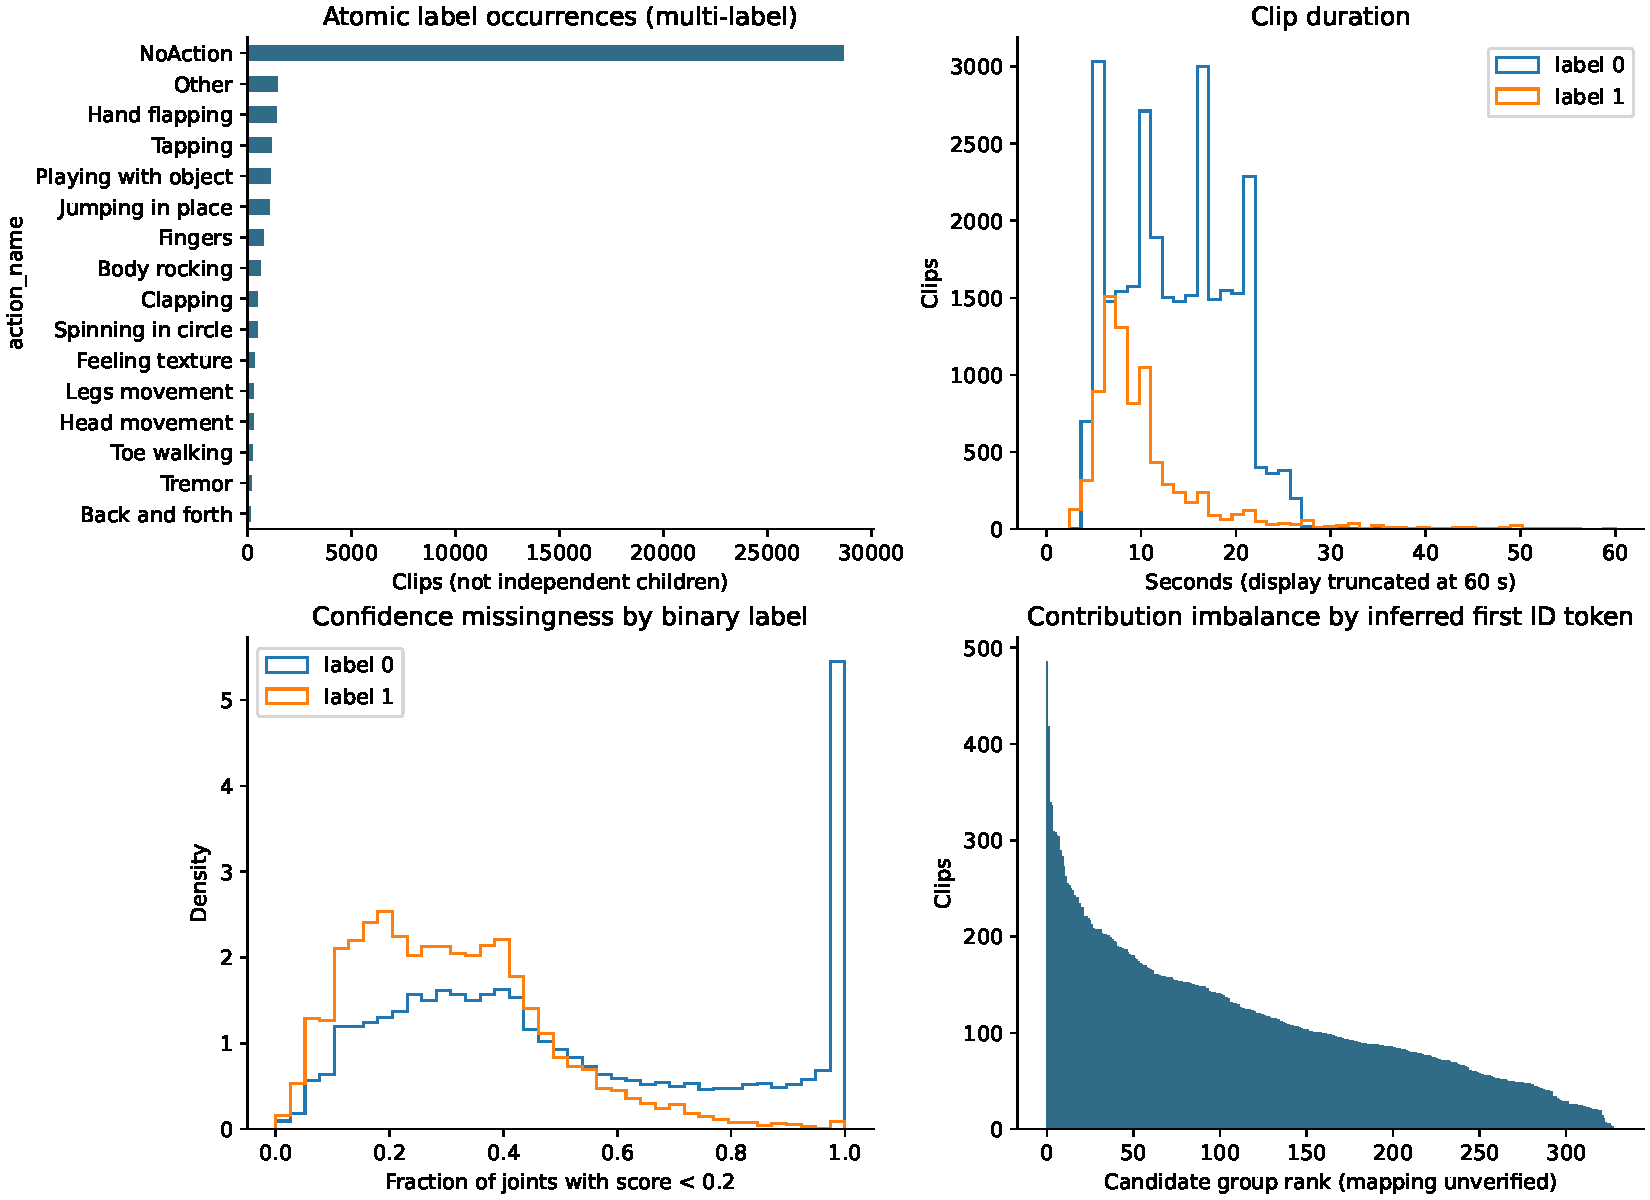
\includegraphics[width=\linewidth]{../../reports/figures/release_overview.pdf}
\caption{Measured release overview. Label counts count atomic names, so combined labels contribute to several categories. The grouping plot uses unverified identifier prefixes. The confidence threshold 0.2 is an audit choice. Duration display is truncated at 60 seconds.}
\end{figure}

\subsection{What is not established by the public clip file}
The inspected records do not contain age, sex, diagnostic scores, medication, individual clinical severity, intervention exposure, a verified participant crosswalk, annotator disagreement or explicit camera calibration. The original paper's cohort-level descriptive statistics cannot be assigned to individual records. Video context, facial expression, detailed finger articulation, sensory triggers and subjective function cannot be reconstructed from 17 body joints. Some of these questions may become possible with additional authorized data, but they are not current measurements. The need for an author-supplied version/split/timing explanation is recorded in \artifact{docs/OPEN_QUESTIONS.md}.
